\section{1D column transport}

File: \texttt{02\_column\_transport.yaml}

\subsection{Description and input}

This is a variant of \texttt{01\_column.yaml}. The user will learn how
to:

\begin{itemize}
\tightlist
\item
  Use flux boundary conditions;
\item
  Set up the advective transport model.
\end{itemize}

For the fluid flow model we change the atmospheric pressure on the
surface to the more realistic infiltration 200 mm/yr (= 6.34e-9 m/s):

\begin{verbatim}
    - region: .surface
      bc_type: total_flux
      bc_flux: 6.34E-09
\end{verbatim}

In the resulting file \texttt{water\_balance.txt} we can see that the
value of the input and output flux changes to 6.34e-8. The visual
results are similar to the case \texttt{01\_column.yaml}.

Next we demonstrate a simulation of the transport of a tracer. The
equation of advective transport (no diffusion/dispersion) is specified
by:

\begin{verbatim}
  solute_equation: !Coupling_OperatorSplitting
    transport: !Solute_Advection_FV
\end{verbatim}

The boundary condition of concentration is prescribed on the surface
region:

\begin{verbatim}
    input_fields:
      - region: .surface
        bc_conc: 100
\end{verbatim}

The default type of boundary condition is \texttt{inflow},
i.e.~prescribed concentration is applied where water flows into the
domain.

We provide the name of the transported substance (in general there can
be multiple transported substances):

\begin{verbatim}
  substances: O-18
\end{verbatim}

The end time of the simulation is set in the section \texttt{time} to
value 1e10 seconds (381 years):

\begin{verbatim}
  time:
    end_time: 1e10
\end{verbatim}

The output files can be generated for specific time values. We set the
time step for output to 1e8 seconds (=3 years and 2 months):

\begin{verbatim}
  output_stream:
    times:
      - step: 1e8
\end{verbatim}

Finally, we turn on computation of mass balance with cumulative sums
over the simulation time interval.

\begin{verbatim}
  balance:
    cumulative: true
\end{verbatim}

\subsection{Results}

The results of the mass balance computation are in the output folder in
the file \texttt{mass\_balance.txt}. The evolution of concentration is
depicted in Figure \ref{fig:transport}. A selected part of numerical
results of mass balance is in the Table \ref{tbl:mass_balance}. On the
region ``.surface'', the mass flux of the tracer is still identical (6 ×
10-6 kg/s). On ``.tunnel'', the mass flux is zero at the beginning and
then it changes within around 100 years to the opposite value of inflow
-6 × 10-6 kg/s. Figure \ref{fig:mass_plot} depicts results from the file
\texttt{mass\_balance.txt} for mass transported through the boundaries
``.surface'' and ``.tunnel'' and in the volume of ``rock''.

\begin{figure}[htbp]
\centering
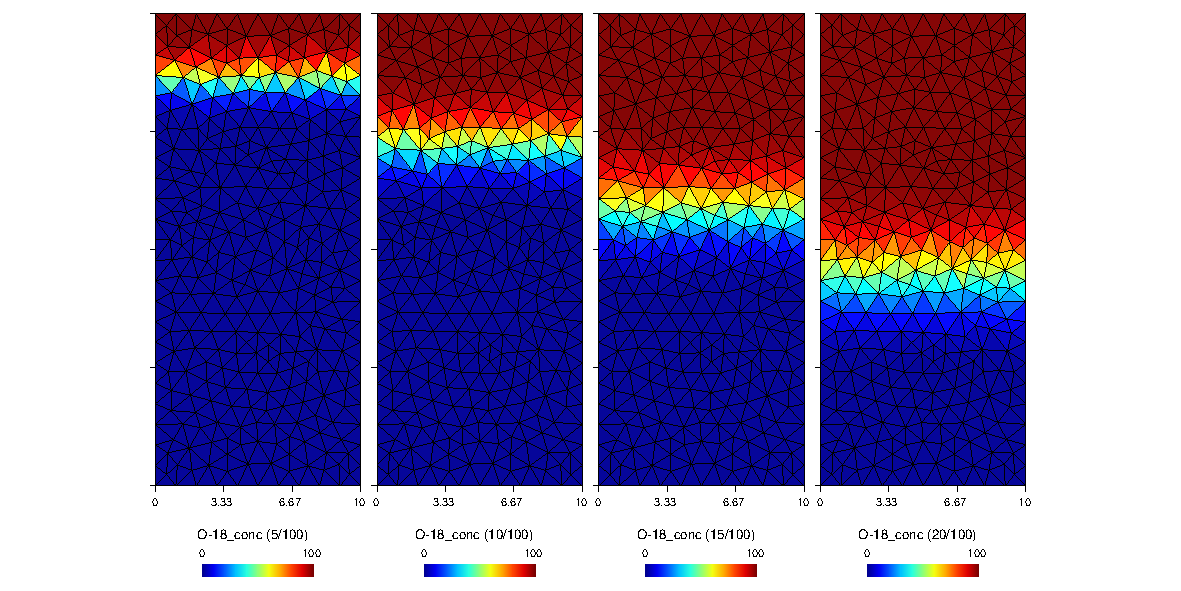
\includegraphics[width=1.00000\textwidth]{tutor_figures/02_transport.pdf}
\caption{Tracer concentration after 5, 10, 15 and 20 time
steps.\label{fig:transport}}
\end{figure}

\begin{longtable}[c]{@{}rllrrrrr@{}}
\caption{Illustration of the results in \texttt{mass\_balance.txt} --
selected columns in two time steps.
\label{tbl:mass_balance}}\tabularnewline
\toprule
time & region & quantity {[}kg{]} & flux & flux\_in & flux\_out & mass &
error\tabularnewline
\midrule
\endfirsthead
\toprule
time & region & quantity {[}kg{]} & flux & flux\_in & flux\_out & mass &
error\tabularnewline
\midrule
\endhead
3.9e+09 & rock & O-18 & 0 & 0 & 0 & 22654.4 & 0\tabularnewline
3.9e+09 & .surface & O-18 & 6.34e-06 & 6.34e-06 & 0 & 0 &
0\tabularnewline
3.9e+09 & .tunnel & O-18 & -4.99e-06 & 0 & -4.99e-06 & 0 &
0\tabularnewline
3.9e+09 & IMPLICIT BOUNDARY & O-18 & -1.02e-19 & 0 & -1.02e-19 & 0 &
0\tabularnewline
3.9e+09 & ALL & O-18 & 1.34e-06 & 6.34e-06 & -4.99e-06 & 22654.4 &
-5.78e-10\tabularnewline
4e+09 & rock & O-18 & 0 & 0 & 0 & 22774.9 & 0\tabularnewline
4e+09 & .surface & O-18 & 6.34e-06 & 6.34e-06 & 0 & 0 & 0\tabularnewline
4e+09 & .tunnel & O-18 & -5.39e-06 & 0 & -5.39e-06 & 0 &
0\tabularnewline
4e+09 & IMPLICIT BOUNDARY & O-18 & -1.02e-19 & 0 & -1.02e-19 & 0 &
0\tabularnewline
4e+09 & ALL & O-18 & 9.40e-07 & 6.34e-06 & -5.39e-06 & 22774.9 &
-6.03e-10\tabularnewline
\bottomrule
\end{longtable}

\begin{figure}[htbp]
\centering
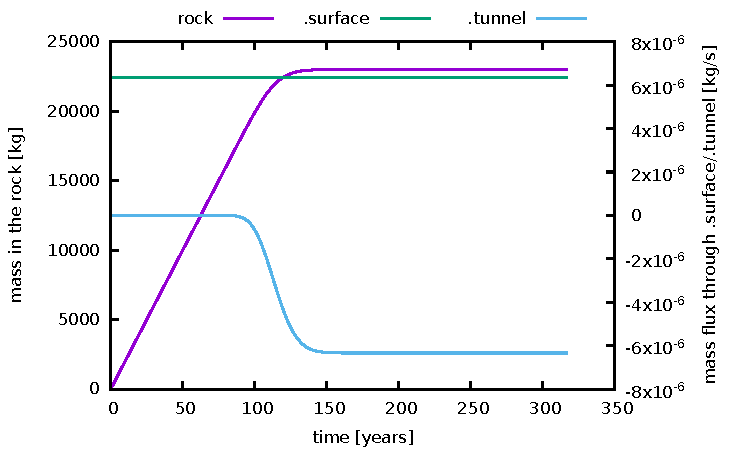
\includegraphics{tutor_figures/02_mass_plot.pdf}
\caption{Results of evolution of mass in the volume and flux through
boundaries.\label{fig:mass_plot}}
\end{figure}
